% !TeX spellcheck = en_US
\chapter{Image Processing}

\section{Linear Filters}
Types of noise:
\begin{itemize}
	\item Salt \& pepper noise
	\item Impulse noise
	\item Gaussian noise\\
	$noise = randn(size(img)) \times \sigma$\\
	$output = img + noise$
	\item \hlr{\underline{Basic assumption:}} \ac{iid}
\end{itemize}
Types of filter:
\begin{itemize}
	\item Correlation Filter: $\displaystyle G[i,j] = \frac{1}{(2k+1)^2} \sum_{u=-k}^{k} \sum_{v=-k}^{k} F[i+u, j+v] $\\
	different weights: $\displaystyle G[i,j] = \sum_{u=-k}^{k} \sum_{v=-k}^{k} H[u,v]F[i+u, j+v] \Rightarrow {\color{red} \boxed{G = H \otimes F}}$\\
	with $H[u,v]$ as non-uniform weights\\
	\hlb{Matlab:} \texttt{filter2, imfilter}
	\item Convolution: \tab $\displaystyle G[i,j] = \sum_{u=-k}^{k} \sum_{v=-k}^{k} H[u,v]F[i-u, j-v] \Rightarrow {\color{red} \boxed{G = H * F}}$\\
	\hlb{Matlab:} \texttt{conv2}\\
	\hlr{If $H[u,v] = H[-u,-v] \Rightarrow$ correlation $\equiv$ convolution}
	\item Averaging Filter: \hlr{Ringing Artifacts??}
	\item Gaussian Filter: $\displaystyle \frac{1}{\sqrt{2\pi}} \exp \left(-\frac{(x-\mu)^2}{2\sigma^2}\right)$\\
	\hlb{Rule of thumb:} set the filter width to $6\sigma$\\
	\hlr{More noise $\Rightarrow\;\; \uparrow \sigma \Rightarrow$ blurring effect}
\end{itemize}

\note
\begin{itemize}
	\item \hlr{$k$ is from the window size $(2k+1)\times(2k+1)$}
	\item \hlr{Efficient implementation:} if filter is separable $\Rightarrow$ apply 1D filter 2 times to have a 2D filter $\Rightarrow$ Reduce the computational cost from $\mathcal{O}(K^2)$ to $\mathcal{O}(2K)$, with $K$ as the kernel size
	\item When coding with \texttt{Python}, the origin of image plane is top left corner, $x$-axis goes left, $y$-axis goes downward (\figref{fig:image-coords})
	\begin{figure}[!htb]
		\centering
		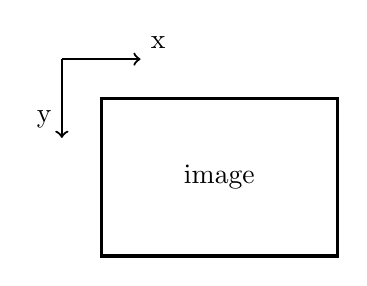
\begin{tikzpicture}			
			\draw[thick,->] (0,0) -- (1,0) node[anchor=south west] {x};
			\draw[thick,->] (0,0) -- (0,-1) node[anchor=south east] {y};
			\draw[very thick] (0.5,-0.5)  rectangle (3.5,-2.5) node[pos=.5]{image};
		\end{tikzpicture}
		\caption{Image coordinate system in \texttt{Python}}	
		\label{fig:image-coords}
	\end{figure}
	\item Boundary issues:
	\begin{align*}
		&\text{- Full: }  \tab \text{output size} = f+g && 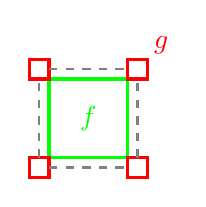
\begin{tikzpicture}[scale=0.5]\draw[green, very thick] (0,0) rectangle (2,2) node[pos=.5]{$f$};
			\draw[red, very thick] (2,2) rectangle (2.5,2.5) node[pos=1.7]{$g$};
			\draw[red, very thick] (0,0) rectangle (-.5,-.5);
			\draw[red, very thick] (2,0) rectangle (2.5,-.5);
			\draw[red, very thick] (0,2) rectangle (-.5,2.5);
			\draw[gray, thick, dashed] (-.25,0) -- (-.25,2);
			\draw[gray, thick, dashed] (0,-.25) -- (2,-.25);
			\draw[gray, thick, dashed] (2.25,0) -- (2.25,2);
			\draw[gray, thick, dashed] (0,2.25) -- (2,2.25);
		\end{tikzpicture}\\
		&\text{- Same:}  \tab \text{output size} = f   && 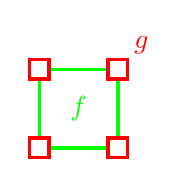
\begin{tikzpicture}[scale=0.5]\draw[green, very thick] (0,0) rectangle (2,2) node[pos=.5]{$f$};
			\draw[red, very thick, fill=white] (1.75,1.75) rectangle (2.25,2.25) node[pos=1.7]{$g$};
			\draw[red, very thick, fill=white] (1.75,-.25) rectangle (2.25,.25);
			\draw[red, very thick, fill=white] (-.25,-.25) rectangle (.25,.25);
			\draw[red, very thick, fill=white] (-.25,1.75) rectangle (.25,2.25);
		\end{tikzpicture}\\
		&\text{- Valid:} \tab \text{output size} = f-g && 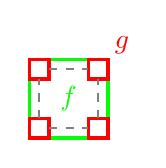
\begin{tikzpicture}[scale=0.5]\draw[green, very thick] (0,0) rectangle (2,2) node[pos=.5]{$f$};
			\draw[red, very thick] (1.5,1.5) rectangle (2,2) node[pos=1.7]{$g$};
			\draw[red, very thick] (0,0) rectangle (.5,.5);
			\draw[red, very thick] (2,0) rectangle (1.5,.5);
			\draw[red, very thick] (0,2) rectangle (.5,1.5);
			\draw[gray, thick, dashed] (.5,.25) -- (1.5,0.25);
			\draw[gray, thick, dashed] (.25,.5) -- (.25,1.5);
			\draw[gray, thick, dashed] (1.75,.5) -- (1.75,1.5);
			\draw[gray, thick, dashed] (.5,1.75) -- (1.5,1.75);
		\end{tikzpicture}
	\end{align*}
	\hlb{Pixel near boundary}:
	\begin{itemize}
		\item Clip filter (black) $\Rightarrow$ dark border
		\item Wrap around
		\item Copy edge $\Rightarrow$ Strong edge response
		\item Reflect across edge
	\end{itemize}
	\item Correlation \ac{vs} convolution:
	\begin{itemize}
		\item Both are linear shift invariant \ac{LSI}:\\
		\tab $h \circ (f_0 + f_1) = h \circ f_1 + h \circ f_0$
		\item Conv is better, it has additional nice properties
		\begin{itemize}
			\item commutative: $f*g = g*f$
			\item associative: $(f*g)*h = f*(g*h)$
			\item Fourier transform $f*g \multimap F.G$ and $f.h \multimap F*H$
		\end{itemize}
		\item With impulse image, Conv reproduces itself, while Corr reflects itself.
	\end{itemize}	
\end{itemize}

\section{Background}
\begin{itemize}
	\item Taking the Fourier Transform of a signal $\Rightarrow$ Frequency coefficients $\Rightarrow$ \hlb{Frequency Spectrum}\\
	\hlr{\underline{Duality:}} $\;$The \hlr{better} a function is \hlr{localized} in one domain\\
	\tab\tab the \hlr{worse} it is \hlr{localized} in the other domain.
	\item Effect of Convolution: $ f * g \multimap F \cdot G$\\
	taking convolution in one domain is equivalent to multiplication in the other domain\\
	A Guassian has compact support in both domains\\
	$\Rightarrow$ \hlb{convenient choice} for \hlr{low-pass filter}
	\item Sharpening filter - \hlr{high-pass filter}: emphasizes noise as well
\end{itemize}
\begin{figure}[!htb]
	\centering
	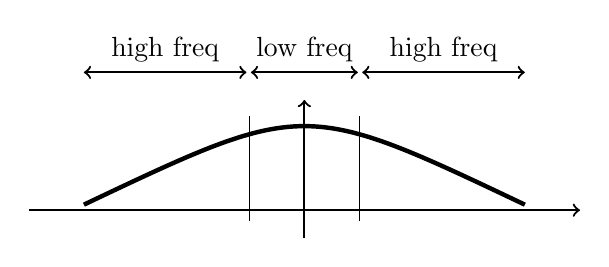
\begin{tikzpicture}[scale=0.7]
		\draw[thick,->] (-5,0) -- (5,0);
		\draw[thick,->] (0,-.5) -- (0,2);
		\draw[ultra thick] (-4,.1) .. controls (0,2) .. (4,.1);
		\draw[thin] (-1,-.2) -- (-1,1.7);
		\draw[thin] (1,-.2)  -- (1,1.7);
		\draw[thick,<->] (-4,2.5) -- (-1.05,2.5) node[pos=0.5, above=0.2]{high freq};
		\draw[thick,<->] (1.05,2.5) -- (4,2.5) node[pos=0.5, above=0.2]{high freq};
		\draw[thick,<->] (-0.97,2.5) -- (0.97,2.5) node[pos=0.5, above=0.2]{low freq};
	\end{tikzpicture}
	\caption{Frequency domain (Fourier).}
	\label{fig:freq-domain}
\end{figure}

\section{Non-Linear Filters}
\begin{itemize}
	\item Median filter: replace each pixel by the median of the neighbors.
	\begin{itemize}
		\item \hlr{remove spikes} (good for impulse, salt \& pepper noise)
		\item \hlr{edge preserving} (unlike mean filter)
	\end{itemize}
	\note If we increase the Median filter's filter size $\Rightarrow$ reduce structure and loose details
\end{itemize}

\section{Multi-Scale Representations}
Image pyramid: very \hlb{little overhead} (in terms of \hlb{computational cost}).

\hlb{Fourier Interpretation:} Discrete Sampling\\
Sampling in spatial domain is like \hlb{multiplying with a spike \ac{func}}.

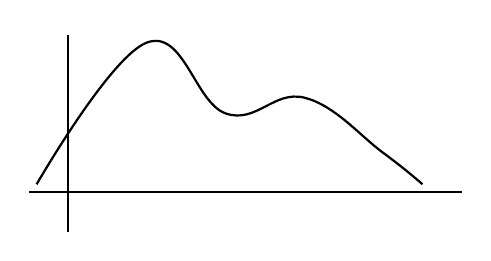
\begin{tikzpicture}
	\draw[thick] (-.5,0) -- (5,0);
	\draw[thick] (0,-.5) -- (0,2);
	\draw[thick] plot [smooth, tension=.7] coordinates {(-.4,.1) (1,1.9) (2,1) (3,1.2) (4, .5) (4.5,0.1)};
\end{tikzpicture}

$\Rightarrow$ Sampling in the frequency domain is like \hlb{convolving with a spike \ac{func}}.

\section{Filters as Templates}
Correlation filtering as Template Matching.

\section{Image Gradients}


\section{Edge Detection}


\section{Structure Extraction}

\todo{missing content}